\subsection{Theoretical predictions for \texorpdfstring{$\pth$}{pTH} as a function of Higgs boson couplings}


% The kinematics of the Higgs boson are fully described by $\mh$, $\absy$ and $\pth$.
% % 
% The $\absy$ distribution is determined mostly by the gluon PDF; while interesting as a potential constrain on the gluon PDF in a global PDF fit, it is of limited value in the context of Higgs boson property measurements.
% % 
% In order for $\pth$ to be non-zero, the production of the Higgs boson has to be associated with some other particle to recoil off of, which naturally occurs via QCD radiation.


% The dominant Higgs boson production mode at the LHC is $\ggh$, and as such the predictions of differential distributions are given primarily by the predictions of $\ggh$.
% % 
% Because of the loop in the LO $\ggh$ diagram, the $\pth$ distribution of Higgs bosons produced via $\ggh$ is a good probe for new physics and potentially a portal towards precision measurements of the Higgs boson properties, for the following reasons.
% % 
% Firstly, up until now, the loop has not been observed experimentally; Confirming its existence is an important verification of the SM.
% % 
% Secondly, the couplings of the Higgs boson to other SM particles can affect the shape of differential distributions while preserving the overall normalization.
% % 
% By fitting the shape of theoretical predictions under simultaneous variations of Higgs boson couplings to the shape observed in data, the Higgs boson couplings can be further constrained.
% % 
% And thirdly, if there any heavy BSM particles in the loop, the tails of the $\pth$ are expected to deviate with respect to their SM values.
% % 
% As the tails concern only a small part of the inclusive cross section, these deviations would be hard to observe in an inclusive cross section measurement.
% % 
% This thesis is concerned with the first two points, although the applied methodology would as well be suitable for a search of heavy particles in the $\ggh$ loop.


% \subsubsection{The low \texorpdfstring{$\pth$}{pTH} regime: variations of \texorpdfstring{$\kappab$}{kb} and \texorpdfstring{$\kappac$}{kc}}

% Light quarks affect the shape of the differential $\pth$ distribution due to interference with the top quark in $\ggh$ production loop.
% % 
% At moderate $\pth$, where the transverse momentum stems from QCD emission with $\mq < \pt^\text{emission} < \mh$ ($\mq$ being the mass of a light quark $\qquark$), the LO calculation of the $\ggh$ production cross section contains terms of the following sort~\cite{Bishara:2016jga}:
% % 
% \begin{linenomath*}
% \begin{equation}
% \kappaq \frac{\mq^2}{\mh^2}
%     \ln^2 \left(
%         \frac{
%             \left( \pt^\text{emission} \right)^2
%             }{
%             m_\mathrm{q}^2
%             }
%         \right)
% \,,
% \end{equation}
% \end{linenomath*}
% % 
% where $\kappaq$ is the coupling of the Higgs boson to $\qquark$.
% % 
% These terms stem from 


% % 
% At moderate $\pth$, $m_\mathrm{q} \ll \pth \ll \mh$ where $m_\mathrm{q}$ is the mass of a light quark $\mathrm{q}$, the LO $\ggh$ production cross section obtains double logarithms depending on the coupling $\kappa_\mathrm{q}$ (the coupling of the Higgs to the light quark $\mathrm{q}$)~\cite{%
% % Baur:1989cm % really not clear how Bishara et al derived it from this paper
% Bishara:2016jga%
% }:
% % 
% \begin{linenomath*}
% \begin{equation}
% \kappa_\mathrm{q} \frac{m_\mathrm{q}^2}{\mh^2}
%     \ln^2 \left(
%         \frac{\pt^2}{m_\mathrm{q}^2}
%         \right)
% \,.
% \end{equation}
% \end{linenomath*}
% % 
% % NOTE: Bishara actually talks about emissions, not pth... 
% % does that matter? Should read paper Baur:1989cm
% % 

% \tk{
% Mention dat fixed-order breaks down in this regime, en dat dus
% resummation nodig is up to all orders in QCD.
% }

% In particular, when emissions have a transverse momen- tump⊥ intherangemQ ≪p⊥ ≪mh,withmQ beingthe internal quark mass, the leading-order (LO) cross section features double logarithms of the form [17]
% OUTP-16-18P, CERN-TH-2016-136, LAPTH-026/16
% m2 􏰌p2 􏰍
% κ Qln2 ⊥ , (1)
% Q m2h m2Q
%   due to the interference between the Q-mediated and the
% top-mediated contributions. These logarithms dynami-
% cally enhance the dependence on the Yukawa modifica-
% tion κQ. 

% ~\cite{Baur:1989cm}.
% % 


\tk{
TODO: I come back to this section once I have written the theory chapter.
% 
I will probably discuss these predictions already there, and will here only refer back to what was already discussed.
% 
As a placeholder, I now included the literal paper text below.
% 
The plots in Figs.~\ref{fig:theories_ktcgkb} and \ref{fig:theories_kbkc} will go into this section, so those I did already include.
}

Differential cross sections may be used to constrain physical parameters.
% 
In the case of Higgs boson production via gluon fusion, finite quark mass effects and moderate variations to Higgs boson couplings may manifest themselves through distortions of the $\pth$ spectrum.
% 
We interpret the $\pth$ spectrum for gluon fusion in terms of modifications of the couplings of the Higgs boson using two models: one tailored to heavy quarks and thus sensitive to effects at high $\pt$~\cite{Grazzini:2017szg,Grazzini:2016paz}, and the other considering the effect of lighter quarks in the gluon fusion loop~\cite{Bishara:2016jga}.
% 
The cross section of Higgs boson production in association with top quarks is taken to scale quadratically with $\kappat$.
% 
The other production processes are taken to be independent of these couplings.
% 
The coupling modifiers are described in the context of the $\kappa$-framework~\cite{LHCHXSWG:YR3}:
% 
\begin{linenomath*}
\begin{equation}
\kappa_{i}^{2} = \frac{y_{i}}{y_{i}^{\text{SM}}}\,,
\end{equation}
\end{linenomath*}
% 
where $y_i$ is the Higgs boson coupling to particle $i$.
% 
The SM value of any $\kappa_i$ is equal to 1.


Recent developments in transverse momentum resummation procedures have allowed more accurate calculations of the $\pth$ spectrum when including the effects of lighter quarks on Higgs boson production via gluon fusion~\cite{Banfi:2013eda,Bozzi:2003jy,Becher:2010tm,Monni:2016ktx}.
% 
The $\pth$ spectrum for gluon fusion has been calculated for simultaneous variations of $\kappac$ and $\kappab$~\cite{Bishara:2016jga}, providing a novel approach to constrain these couplings via the $\pth$ spectrum.
% 
We parameterize the variations computed in Ref.~\cite{Bishara:2016jga} with a quadratic polynomial for each bin of the differential production cross section, including an inhomogeneity due to the interference of the top quark loop with that from the bottom and charm quarks in the gluon fusion production loop.
% 
The Higgs boson coupling to the top quark is fixed to its SM value in this model.
% 
The calculations from Ref.~\cite{Bishara:2016jga} are given up to the scale of the Higgs mass, and thus the $\hbb$ channel (for which the lower limit of the $\pth$ spectrum is $350$\GeV) is not used as input for the results obtained with this model.


A second model producing simultaneous variations of $\kappat$, $\cg$, and $\kappab$ by adding dimension-6 operators to the SM Lagrangian has been built in Refs.~\cite{Grazzini:2017szg,Grazzini:2016paz}.
% 
This study employs an analytic resummation performed up to next-to-next-to-leading-logarithmic (NNLL) order in order to obtain the $\pth$ spectrum at next-to-NLO+NNLL accuracy.
% 
The dimension-6 operator whose coefficient is $\cg$ yields a direct coupling of the Higgs field to the gluon field with the same underlying tensor structure as in the heavy-top mass limit.
% 
In the SM, the value of $\cg$ equals 0.
% 
The derivation of $\cg$ is given in Ref.~\cite{Grazzini:2017szg} and the inclusive cross section is given by $\sigma \simeq \left| 12\cg + \kappat \right|^2 \sigma^\text{SM}$.
% 
Two other operators are included to describe modifications of $\kappat$ and $\kappab$.
% 
While the model allows simultaneous variation of all three coupling modifiers, we consider only simultaneous variations of $\kappat$ and $\cg$, and of $\kappat$ and $\kappab$.
% 
The precomputed spectra are taken as input from Ref.~\cite{Grazzini:2017szg} and are parametrized using a quadratic polynomial, neglecting the interference of the bottom and top quarks in the gluon fusion loop.





% img/interpretation/other/varparcomp_kbkc.pdf
% img/interpretation/other/varparcomp_ktcg.pdf
% img/interpretation/other/varparcomp_ktkb.pdf


\begin{figure}[hbtp]
  \begin{center}
    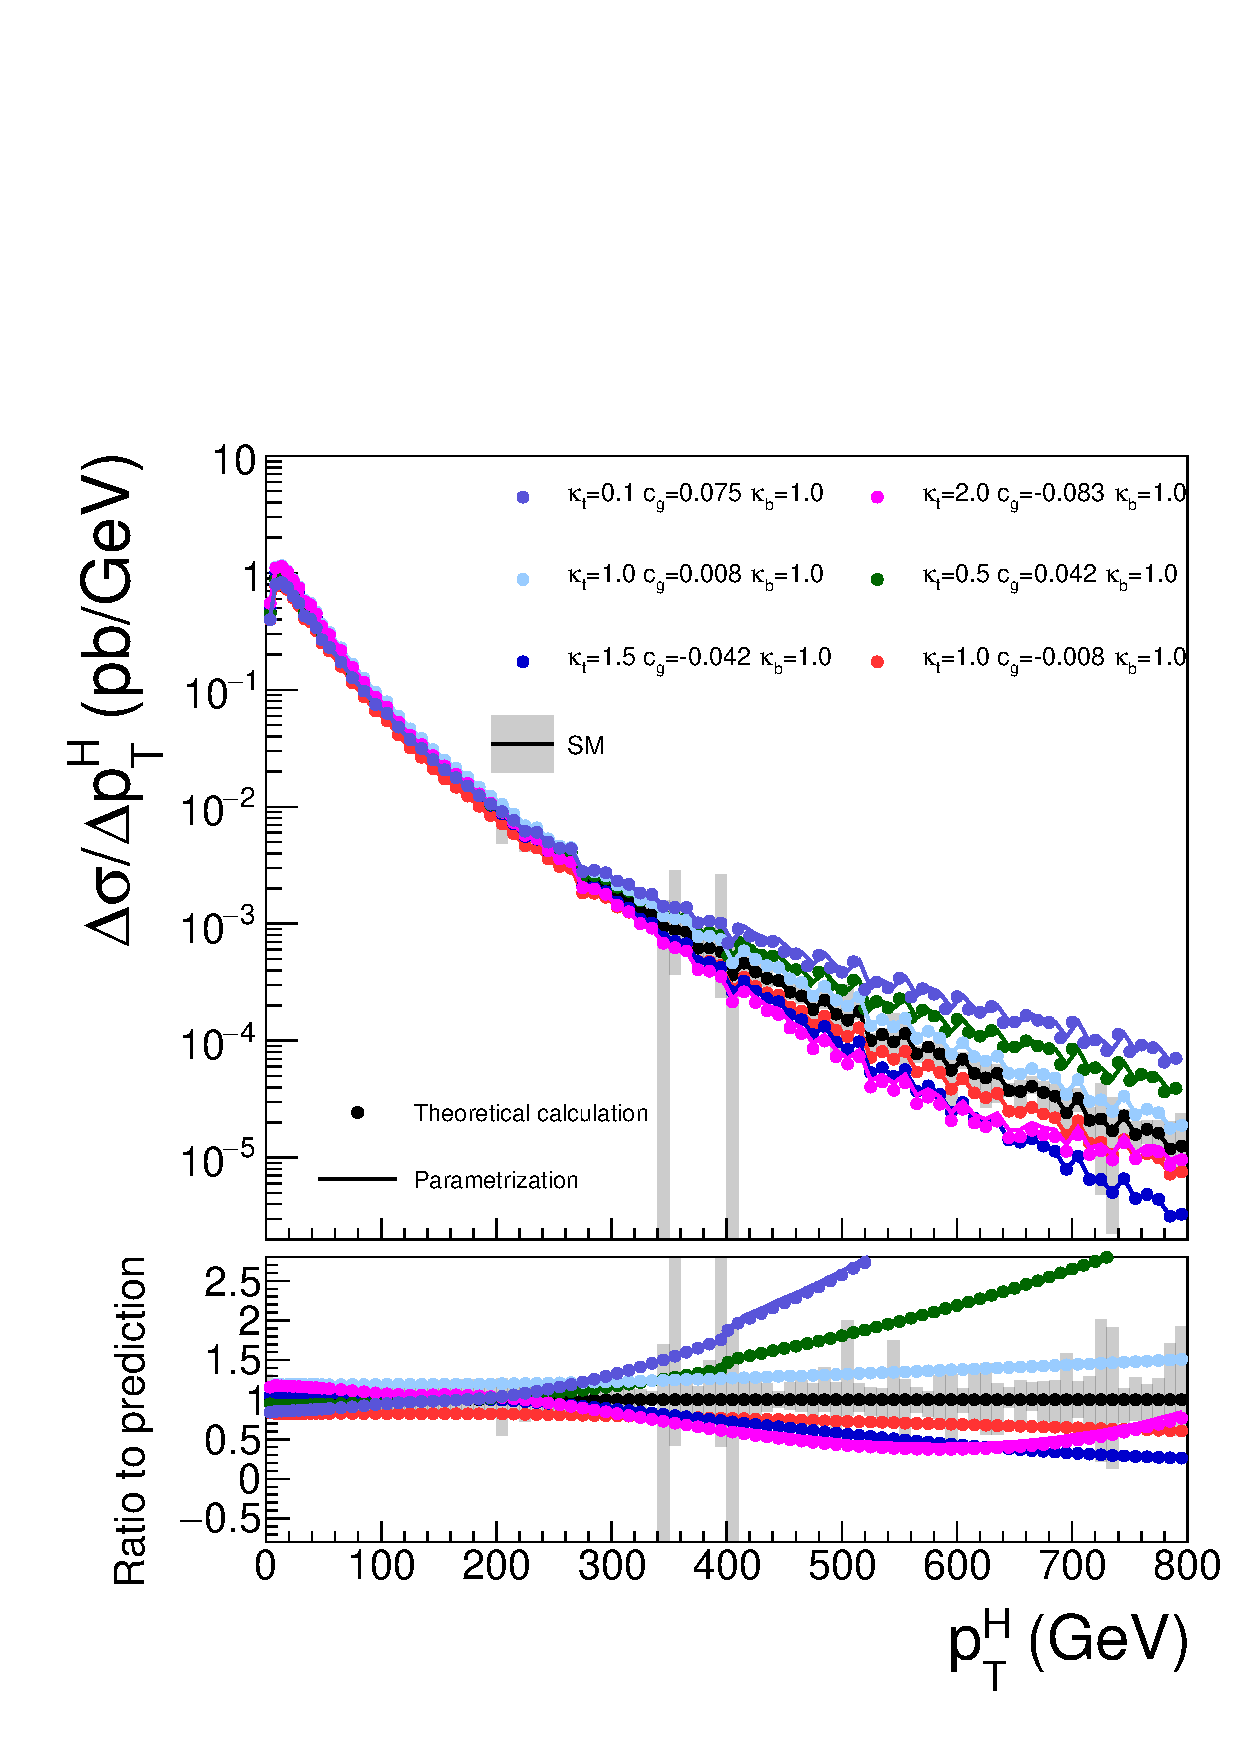
\includegraphics[width=\halflinewidth]{img/interpretation/other/varparcomp_ktcg.pdf}
    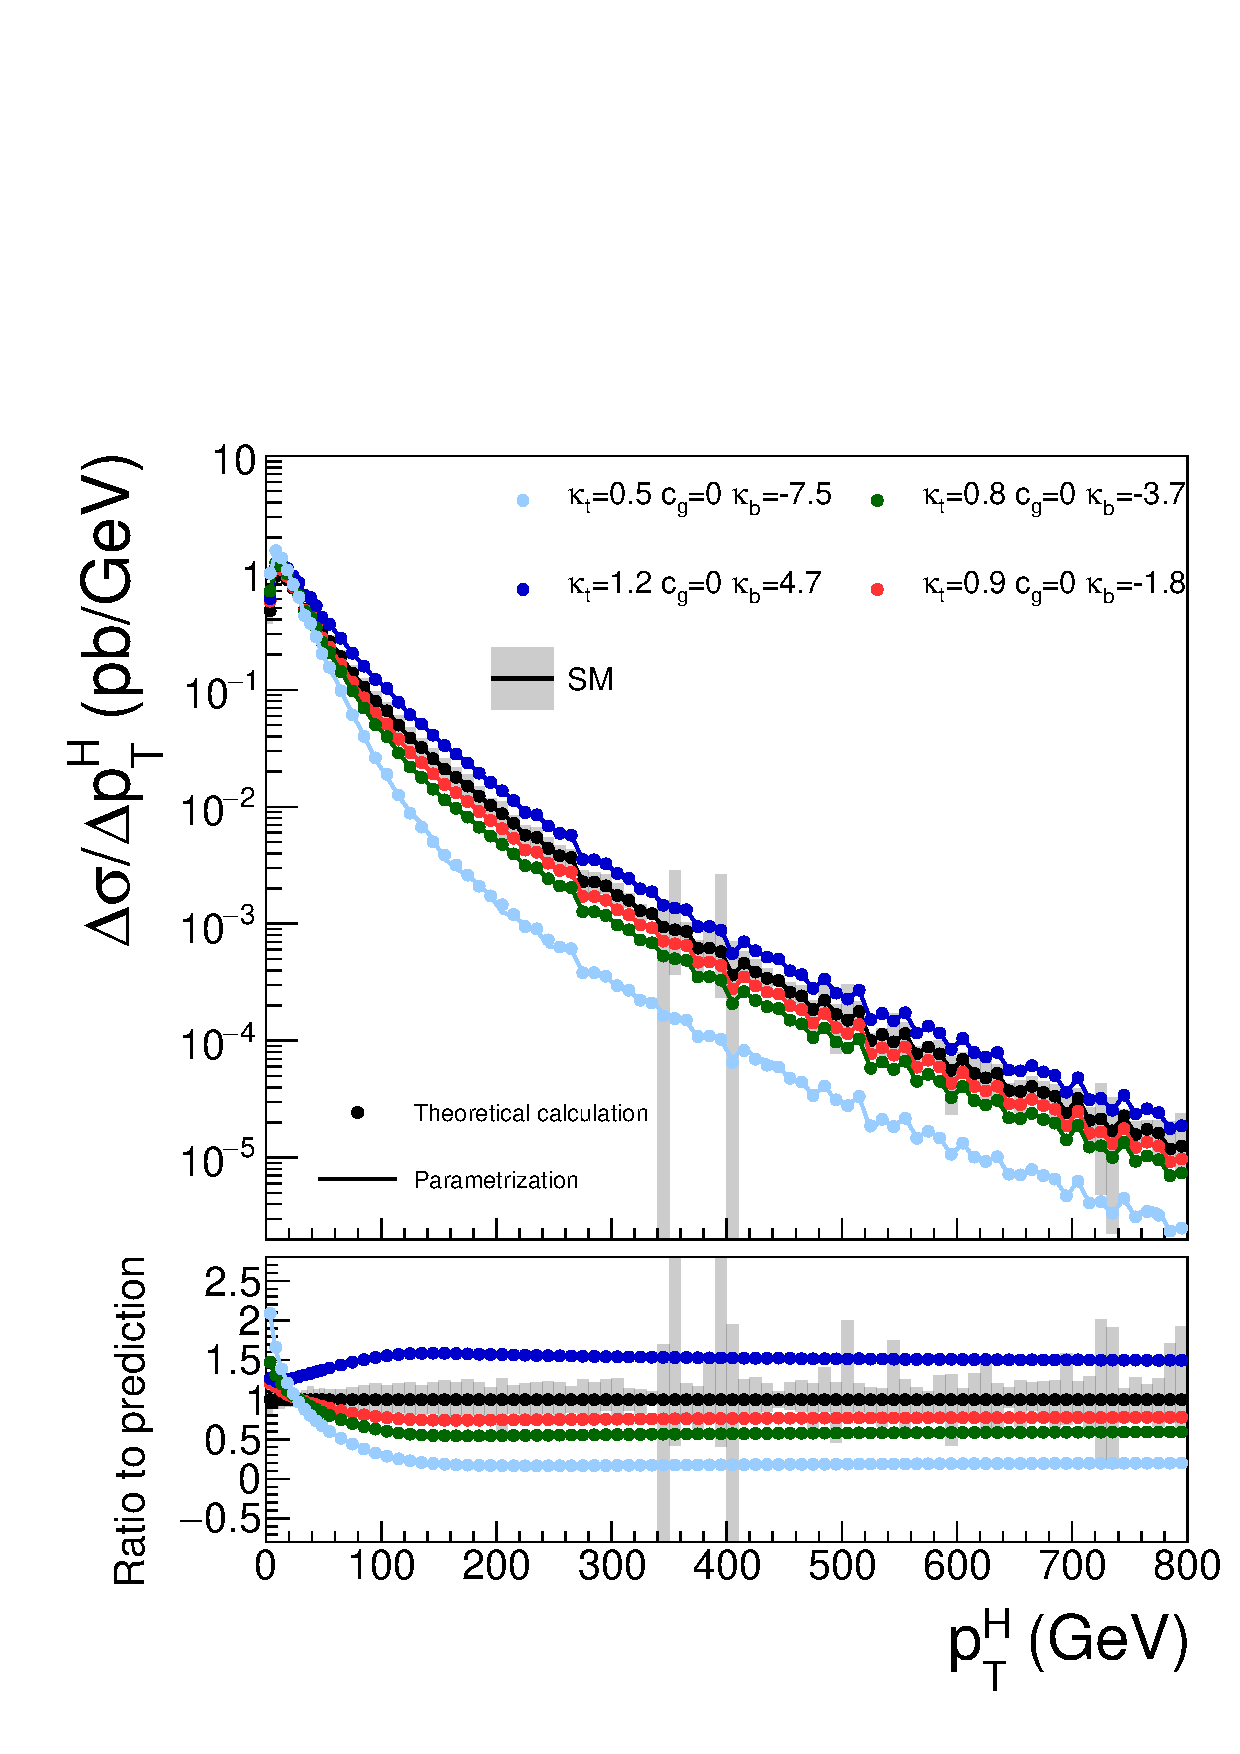
\includegraphics[width=\halflinewidth]{img/interpretation/other/varparcomp_ktkb.pdf}
    % 
    \caption{
        The predicted $\pth$ spectrum for simultaneous variations of $\kappat$ and $\cg$ (left) and $\kappat$ and $\kappab$ (right).
        % 
        The dots correspond to the theoretical calculations performed by the authors in Ref.~\cite{Grazzini:2017szg}, and the corresponding line shows the outcome of the parametrization of the theoretical calculations using a quadratic polynomial.
        % 
        The parametrization matches the exact calculations to a good approximation.
        % 
        The SM prediction is shown in black, with the gray bar indicating the uncertainty due to missing higher order corrections.
        }
    \label{fig:theories_ktcgkb}
  \end{center}
\end{figure}


\begin{figure}[hbtp]
  \begin{center}
    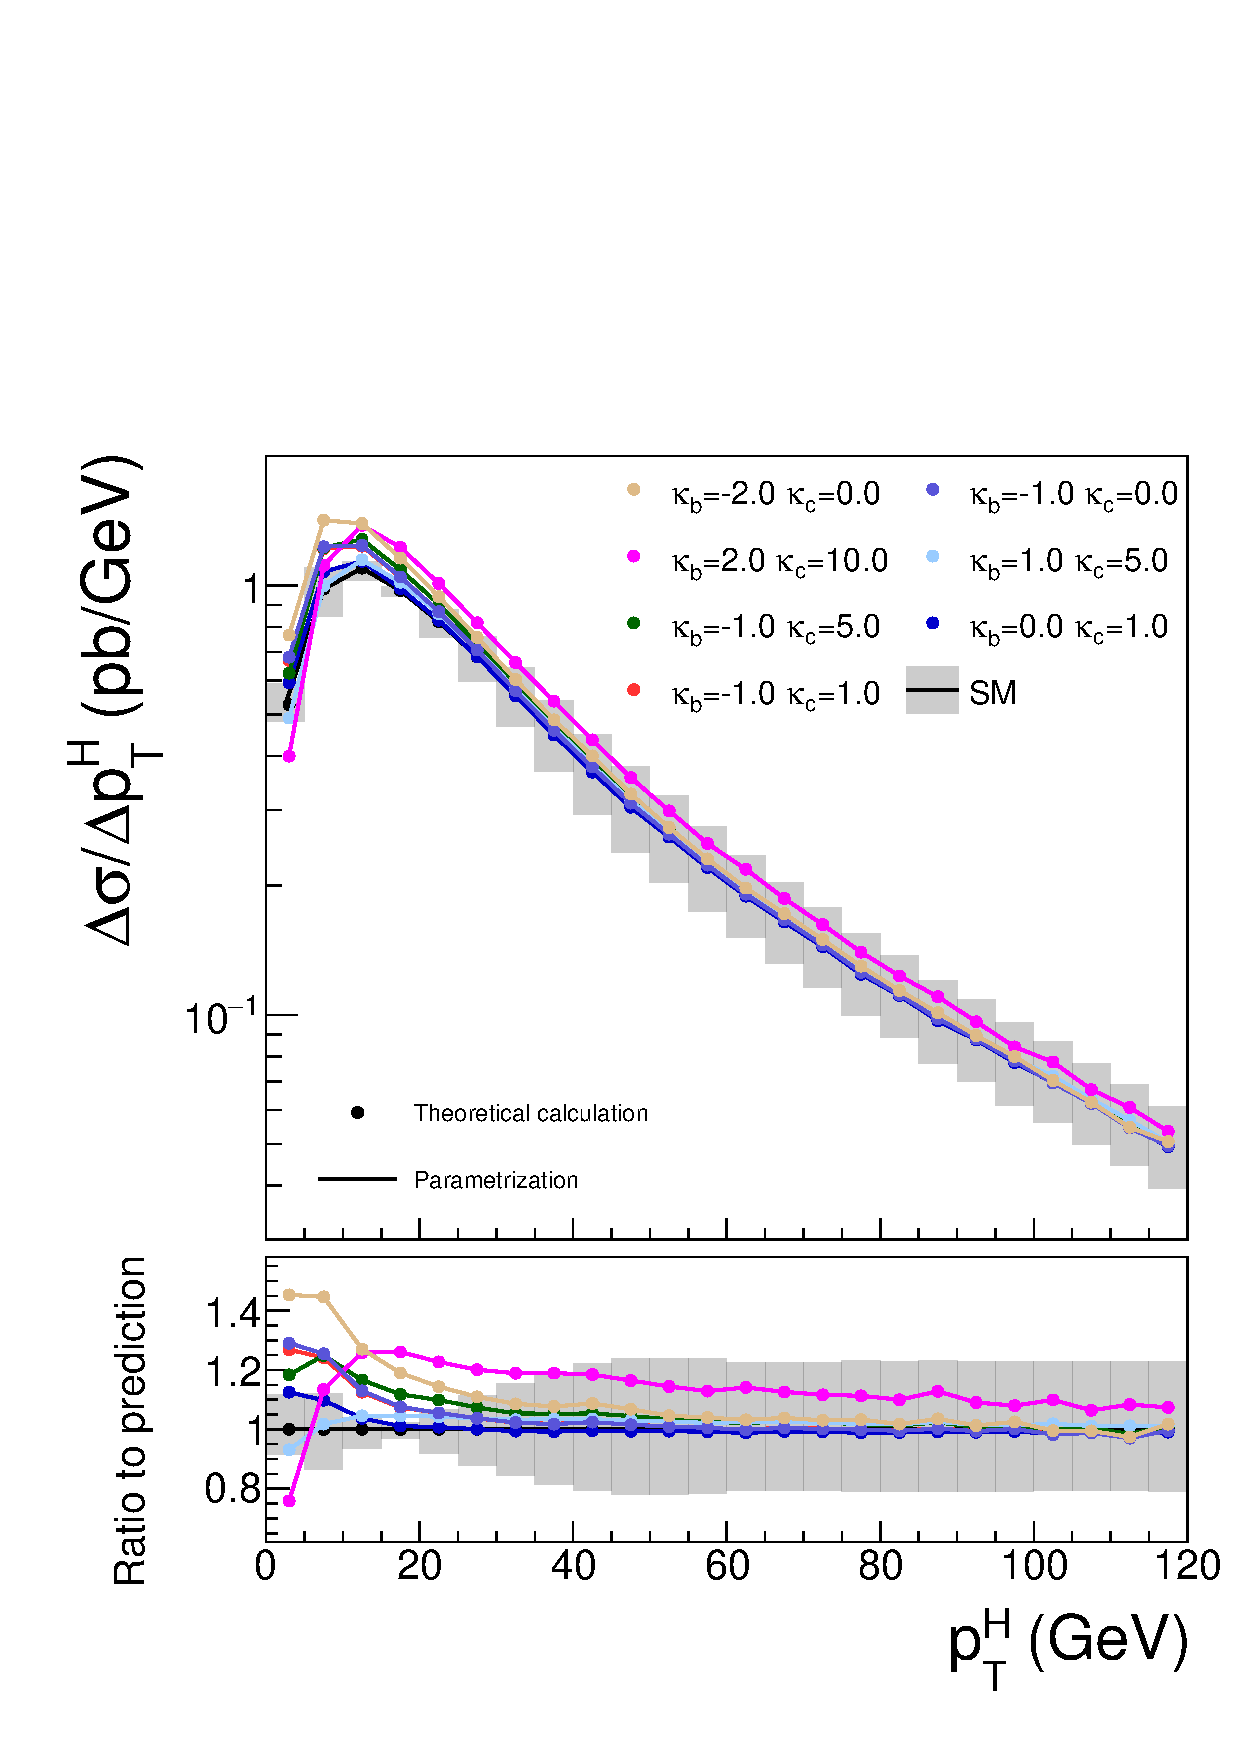
\includegraphics[width=\halflinewidth]{img/interpretation/other/varparcomp_kbkc.pdf}
    % 
    \caption{
        The predicted $\pth$ spectrum for simultaneous variations of $\kappab$ and $\kappac$.
        % 
        The dots correspond to the theoretical calculations performed by the authors in Ref.~\cite{Bishara:2016jga}, and the corresponding line shows the outcome of the parametrization of the theoretical calculations using a fitted quadratic polynomial.
        % 
        The parametrization matches the exact calculations to a good approximation.
        % 
        The SM prediction is shown in black, with the gray bar indicating the uncertainty due to missing higher order corrections.
        }
    \label{fig:theories_kbkc}
  \end{center}
\end{figure}



